\documentclass[border=15pt, multi, tikz]{standalone}
\usepackage{import}
\subimport{./layers/}{init}
\usetikzlibrary{positioning}
\usetikzlibrary{3d} %for including external image 

\def\ConvColor{rgb:yellow,5;red,2.5;white,5}
\def\ConvReluColor{rgb:yellow,5;red,5;white,5}
\def\PoolColor{rgb:red,1;black,0.3}
\def\DcnvColor{rgb:blue,5;green,2.5;white,5}
\def\SoftmaxColor{rgb:magenta,5;black,7}
\def\SumColor{rgb:blue,5;green,15}

\begin{document}
\begin{tikzpicture}

\tikzstyle{connection}=[ultra thick,every node/.style={sloped,allow upside down},draw=\edgecolor,opacity=0.7]

% Input
\node[canvas is zy plane at x=0] (temp) at (-3,0,0) {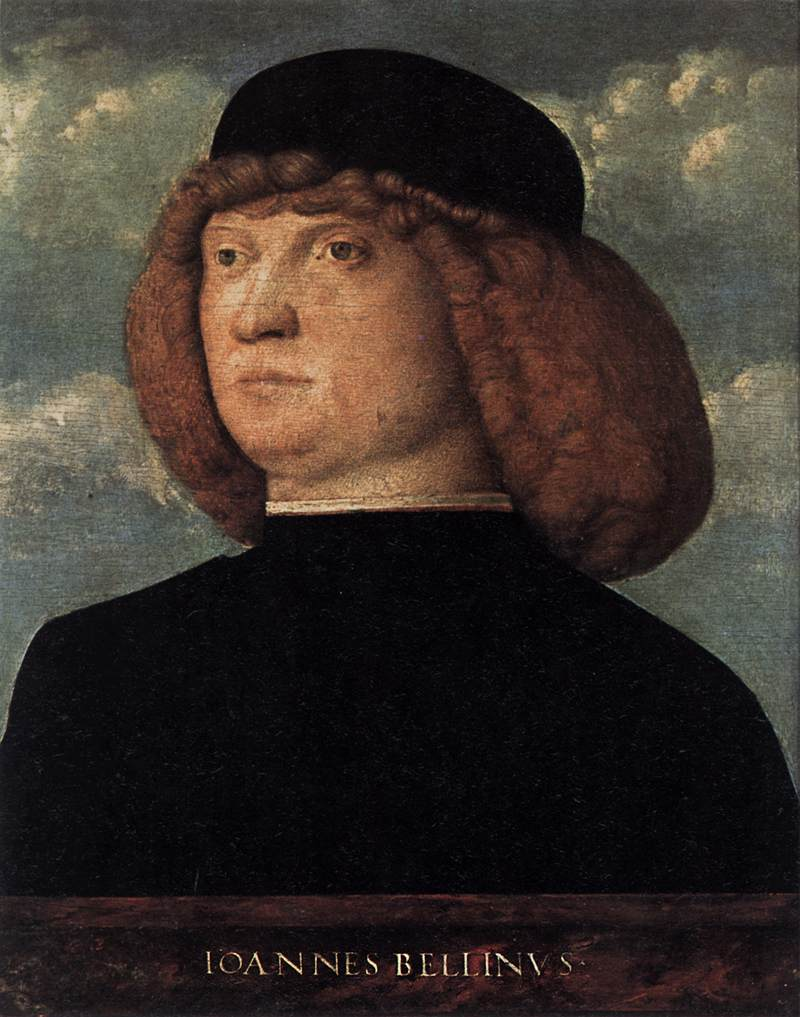
\includegraphics[width=8cm,height=8cm]{543.jpg}};

% Convolutional Blocks
\foreach \i/\j in {1/3,2/16,3/32,4/64}
{
  \pic[shift={(2*\i,0,0)}] at (0,0,0) {RightBandedBox={name=cr\i,caption=conv\i,%
        xlabel={{"\j","\j"}},zlabel=I,fill=\ConvColor,bandfill=\ConvReluColor,%
        height=40,width={2,2},depth=40}};
  \pic[shift={(0,0,0)}] at (cr\i-east) {Box={name=p\i,%
        fill=\PoolColor,opacity=0.5,height=35,width=1,depth=35}};
}

% Adaptive Average Pooling & Flatten
\pic[shift={(0,0,0)}] at (p4-east) {Box={name=adaptive_pool,%
        fill=\PoolColor,opacity=0.5,height=30,width=1,depth=30,caption=Adaptive Avg Pool}};
\pic[shift={(0,0,0)}] at (adaptive_pool-east) {Box={name=flatten,%
        fill=\PoolColor,opacity=0.5,height=25,width=1,depth=25,caption=Flatten}};

% Fully Connected Layers
\pic[shift={(2,0,0)}] at (flatten-east) {RightBandedBox={name=fc1,caption=FC,%
        xlabel={{"64","128"}},zlabel=I,fill=\ConvColor,bandfill=\ConvReluColor,%
        height=20,width={2,2},depth=20}};
\pic[shift={(2,0,0)}] at (fc1-east) {RightBandedBox={name=fc2,caption=FC,%
        xlabel={{"64","12"}},zlabel=I,fill=\ConvColor,bandfill=\ConvReluColor,%
        height=15,width={2,2},depth=15}};

% Connections
\draw [connection]  (p1-east) -- node {\midarrow} (cr2-west);
\draw [connection]  (p2-east) -- node {\midarrow} (cr3-west);
\draw [connection]  (p3-east) -- node {\midarrow} (cr4-west);
\draw [connection]  (p4-east) -- node {\midarrow} (adaptive_pool-west);
\draw [connection]  (adaptive_pool-east) -- node {\midarrow} (flatten-west);
\draw [connection]  (flatten-east) -- node {\midarrow} (fc1-west);
\draw [connection]  (fc1-east) -- node {\midarrow} (fc2-west);

\end{tikzpicture}
\end{document}
